% !TeX encoding=unicode
% !TeX spellcheck = de-DE

\chapter{Experimentelle Vorgehensweise}
\section{???}
\label{sec:xtransform}
\appl{} and \fnlo{} do not use the momentum fraction $x$ and the factorization scale $Q^2$ directly in their grids.
Instead they provide transformations that are supposed to achieve better coverage of the values.
In the following we will concentrate on the $x$ distribution, which is more crucial to the number of grid points needed.
The functions provided by \appl{} are:
%
\begin{align}
	f_0(x)	&= \log(\frac{1}{x} -1) \\
	f_1(x)	&= -\log(x) \\
	f_2(x)	&= \sqrt{-\log(x)} \\
	f_3(x)	&= -\log(x) + 5 \cdot (1-x) \, .
\end{align}
%
\fnlo{} only provides the functions $f_1(x)$ and $f_2(x)$.
To be used in a grid, the functions are divided into equal-sized bins.
In order to avoid empty bins, the limit values are determined in a seperate \enquote{phasespace run} before the actual fill run.

The functions (normalized to the domain $[0,1]$ for comparability) are shown in \figref{fig:xtransform}.
%
\begin{figure}[]
	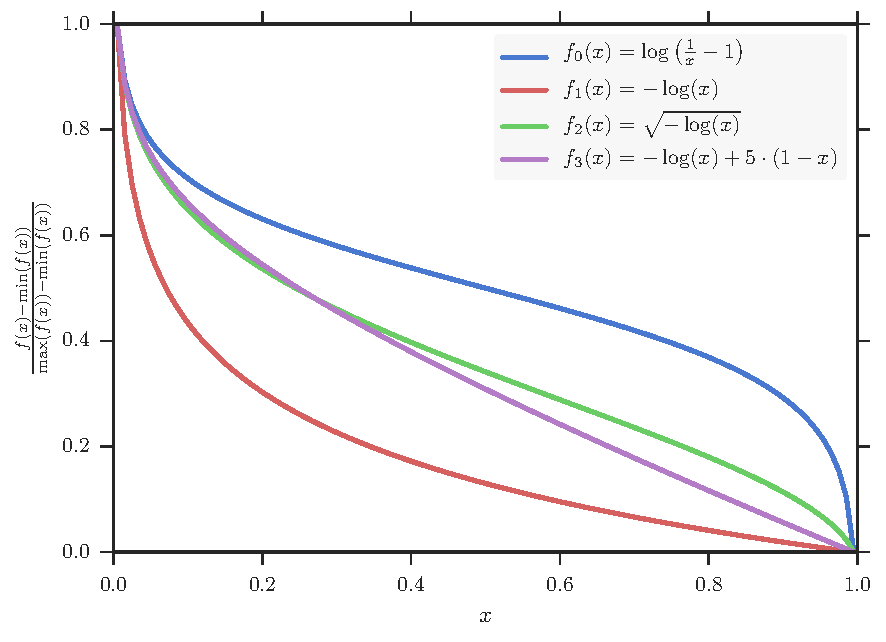
\includegraphics[width=0.7\textwidth]{images/xtransform.pdf}
	\caption{The transformations applied to the $x$ distribution, normalized to the range $[0,1]$.}
	\label{fig:xtransform}
\end{figure}
%
All transformations increase the point density in the low $x$ region, where most events should fall into.
Compared against $f_0$, the other functions also accomplish a higher point density in the high $x$ region.
Some observables in specific processes might benefit from this.

We can look at the actual $x$ distribution in the process considered in this thesis.
In \figref{fig:x_compare} it is plotted for one of the gluons involved in the process $gg \rightarrow H + j$ at leading order for a center-of-mass energy of $\sqrt{s} = \SI{13}{\tera\electronvolt}$.
For comparison, the respective distribution for the functions $f_1$ to $f_4$ is also shown.
In the bare distribution, the number of events per bin increases rapidly towards low $x$.
It is obvious that the reproduction of the low $x$ region is poor for this linear binning.
We expect that for some $x>0$ the number of events approaches zero, because there has to be at least enough momentum transfer to produce the Higgs boson and the jet.
To see this with linear binning, one would need a huge amount of bins.
In contrast, the transformations are able to project the low $x$ peak to a higher number of bins than the naive linear binning.
Additionally, they all approach zero for a finite value (note that high values of $f(x)$ correspond to low values of $x$).
Due to the normalization, this happens at $1$.
For all transformed distributions, it should be possible to interpolate them with a reasonable number of sampling points.
The function $f_1(x)$ looks most promising, as it allocates many bins for the peak region, which should be the most relevant for this process.

%
\begin{figure}[]
	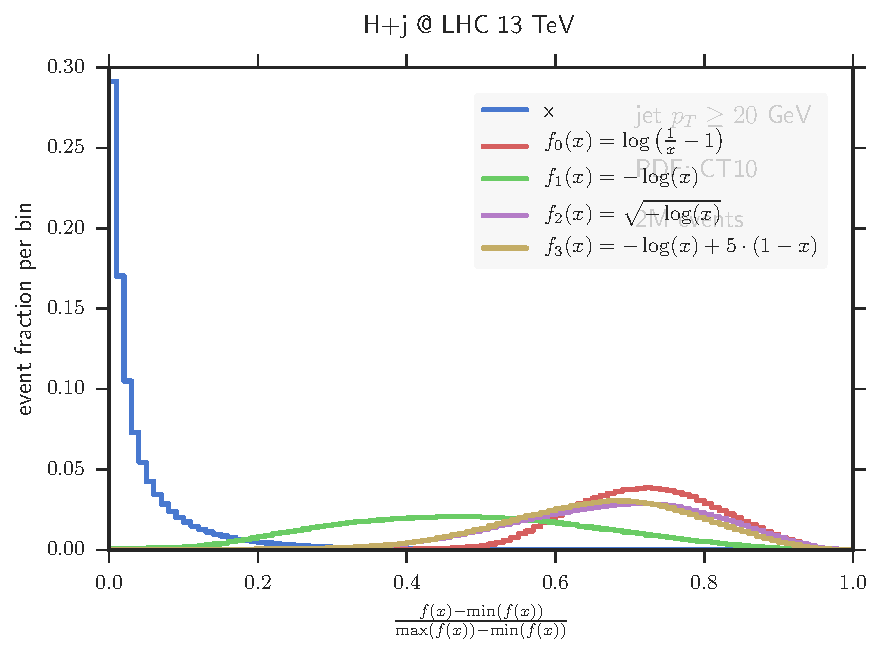
\includegraphics[width=0.7\textwidth]{images/x_compare.pdf}
	\caption{The event fraction per bin for the different transformations.}
	\label{fig:x_compare}
\end{figure}
%

If we want to be more specific, we can extract the dependence of the observables on $x$ and $f(x)$, respectively, from the generated events.
This is shown in \figref{fig:hpt_compare} for the transverse momentum $p_\perp$ and in \figref{fig:hy_compare} for the rapidity $y$ of the Higgs boson.
For both observables all considered functions are reasonable.
Again, the function $f_1(x)$ seems to be best suited.
Hence, it will be the transformation used in all following grid calculations.
%
\begin{figure}[]
	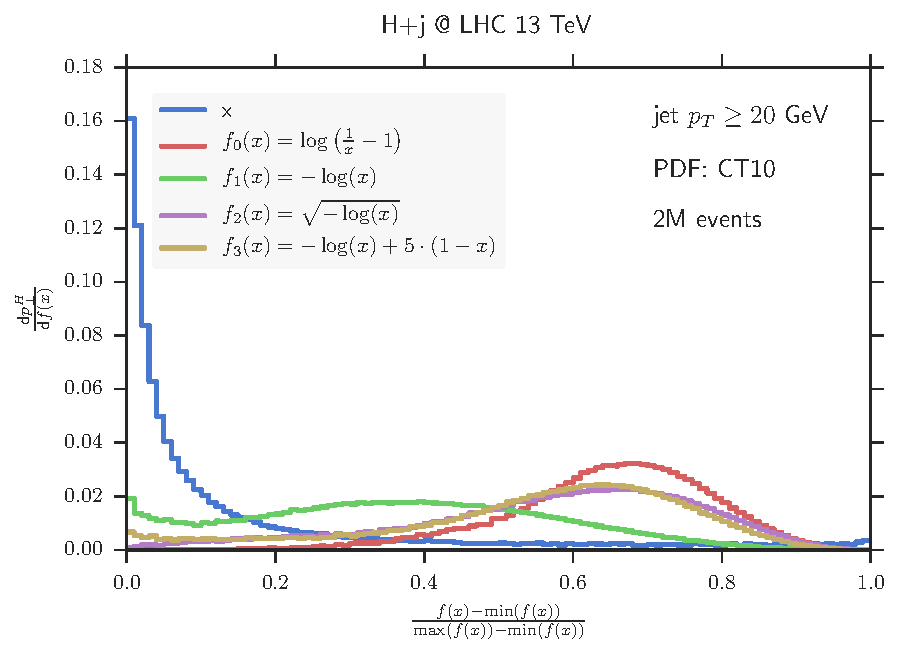
\includegraphics[width=0.7\textwidth]{images/hpt_compare.pdf}
	\caption{The transverse momentum $p_\perp$ of the Higgs boson differential in f(x).
				The ordinate shows the fraction per bin.}
	\label{fig:hpt_compare}
\end{figure}
%
%
\begin{figure}[]
	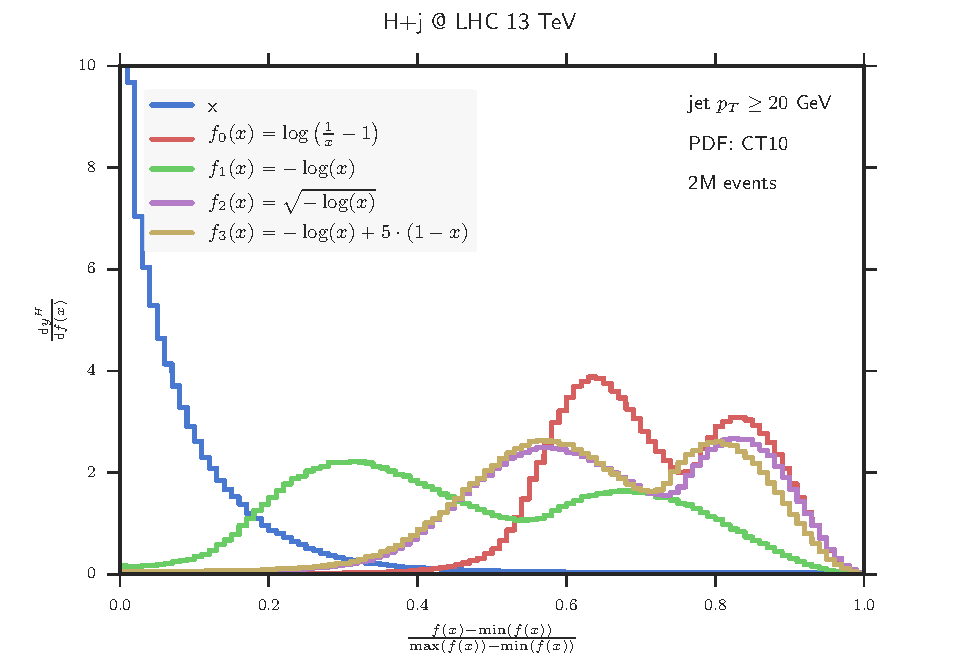
\includegraphics[width=0.7\textwidth]{images/hy_compare.pdf}
	\caption{The rapidity $y$ of the Higgs boson differential in f(x).
				The ordinate shows the fraction per bin.}
	\label{fig:hy_compare}
\end{figure}
%
